\clearpage
\appendix

% all of this just to remove a page number :)
\begingroup
\makeatletter
\let\ps@plain\ps@empty
\appendixpage
\makeatother
\endgroup


\chapter{Diagramas de Gantt}
\section{Diagrama de Gantt de la planificación inicial} \label{appendix:a}
\begin{figure}[H]
\centering
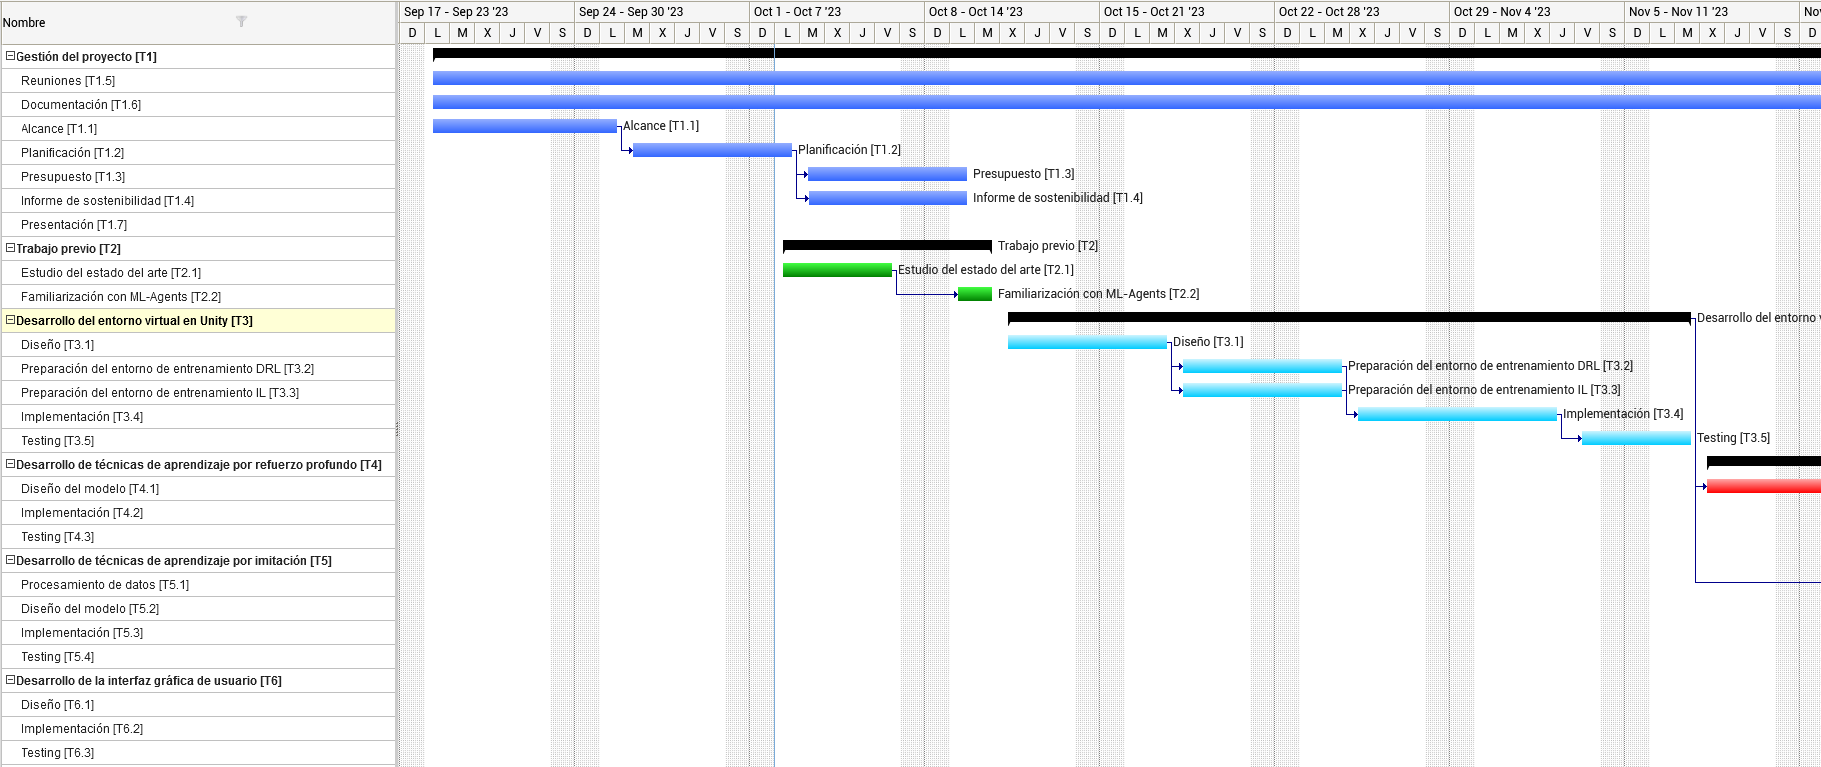
\includegraphics[width=\textwidth]{figures/gantter1.png}
\caption[Diagrama de Gantt de la planificación inicial, parte 1 de 2]{Diagrama de Gantt de la planificación temporal, parte 1 de 2. (Elaboración propia)}
\label{fig:gantter1}
\end{figure}

\begin{figure}[H]
\centering
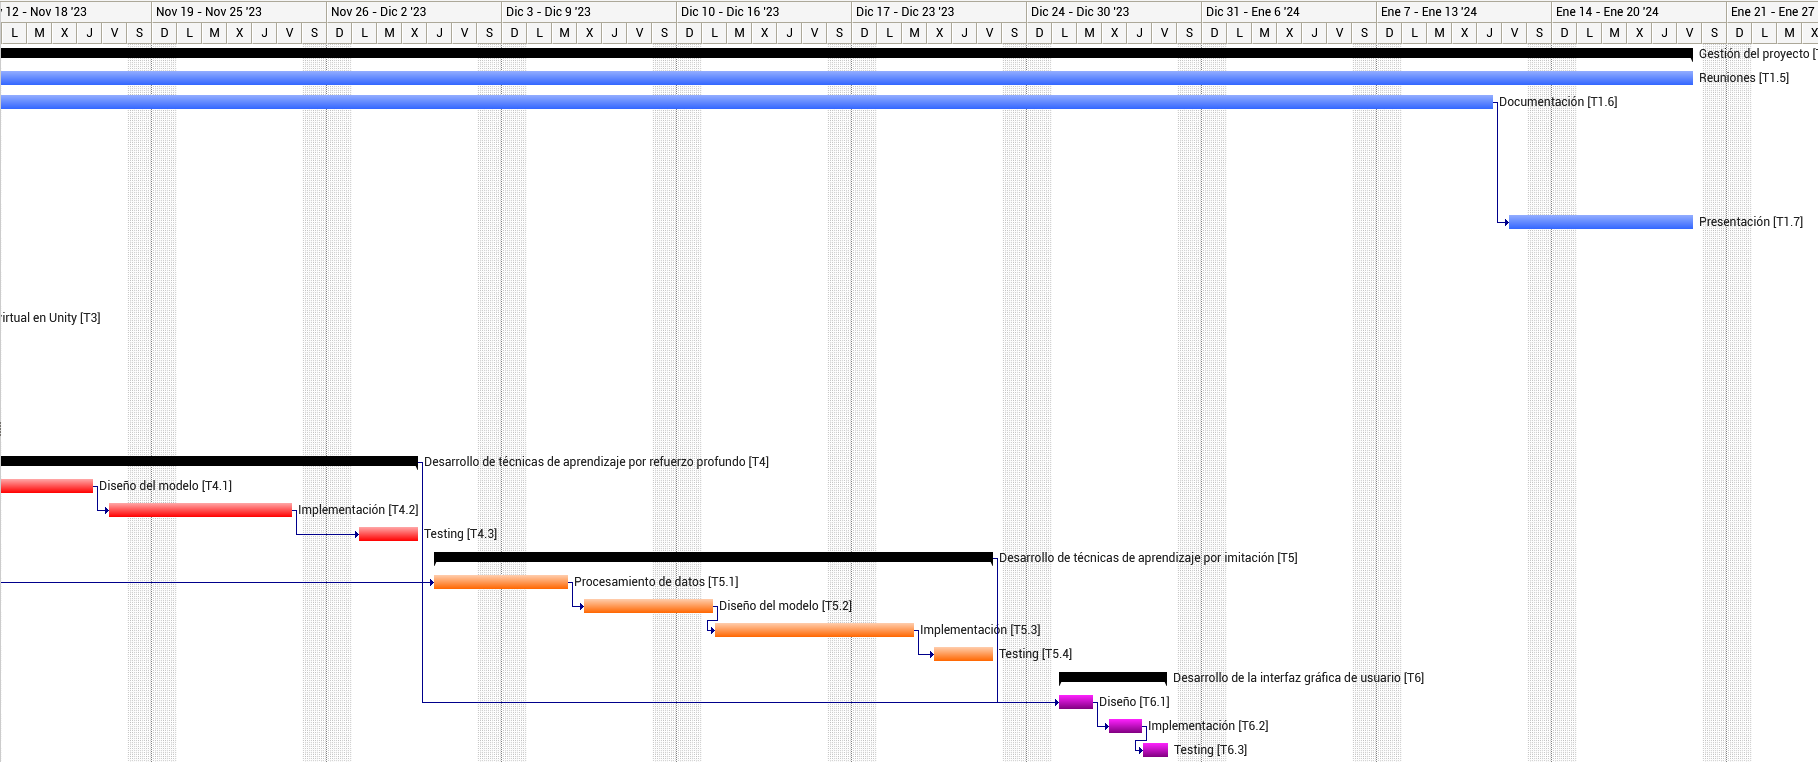
\includegraphics[width=\textwidth]{figures/gantter2.png}
\caption[Diagrama de Gantt de la planificación inicial, parte 2 de 2]{Diagrama de Gantt de la planificación temporal, parte 2 de 2. (Elaboración propia)}
\label{fig:gantter2}
\end{figure}

\newpage

\section{Diagrama de Gantt de la planificación final}\label{appendix:b}

\begin{figure}[H]
\centering
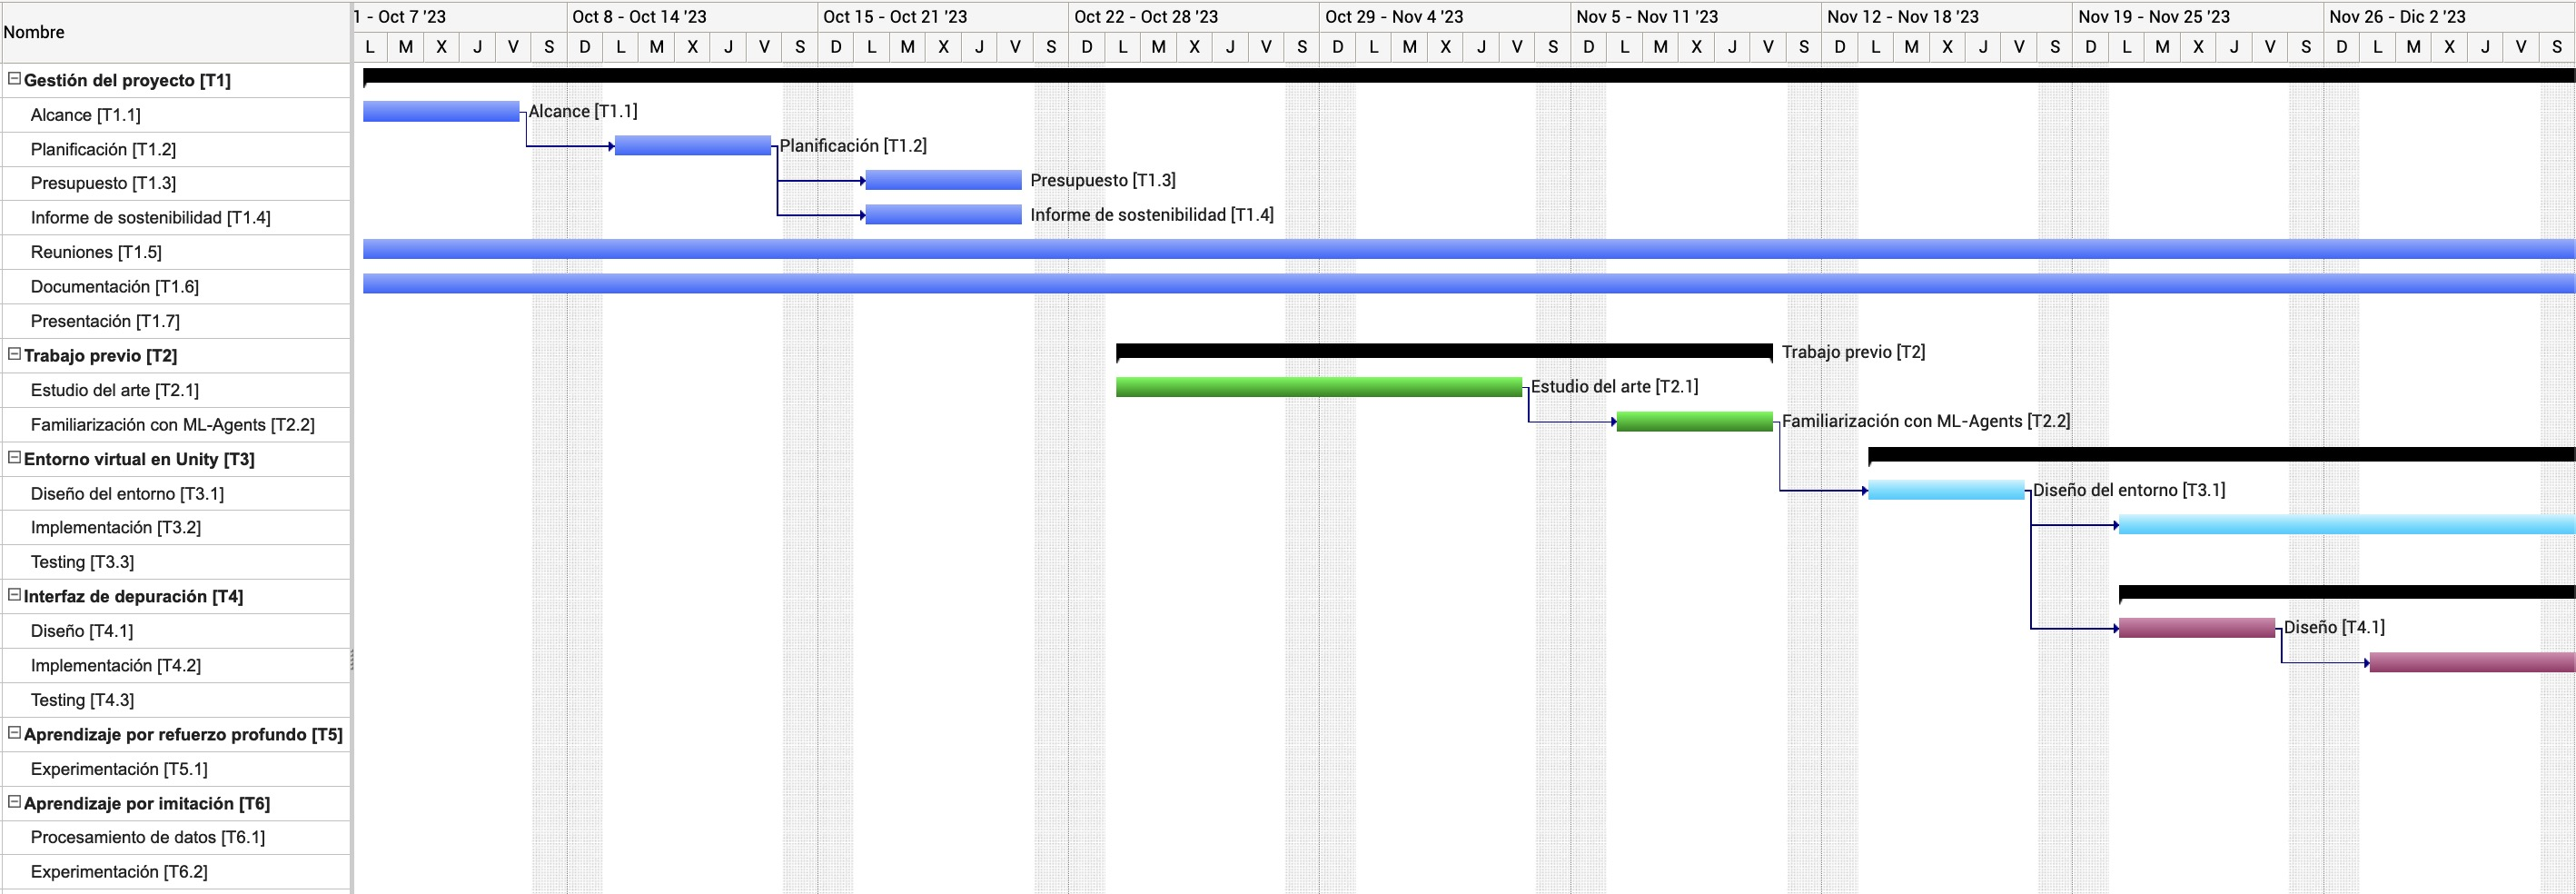
\includegraphics[width=\textwidth]{figures/gantter1-final.jpg}
\caption[Diagrama de Gantt de la planificación final, parte 1 de 2]{Diagrama de Gantt de la planificación final, parte 1 de 2. (Elaboración propia)}
\label{fig:gantter1-final}
\end{figure}

\begin{figure}[H]
\centering
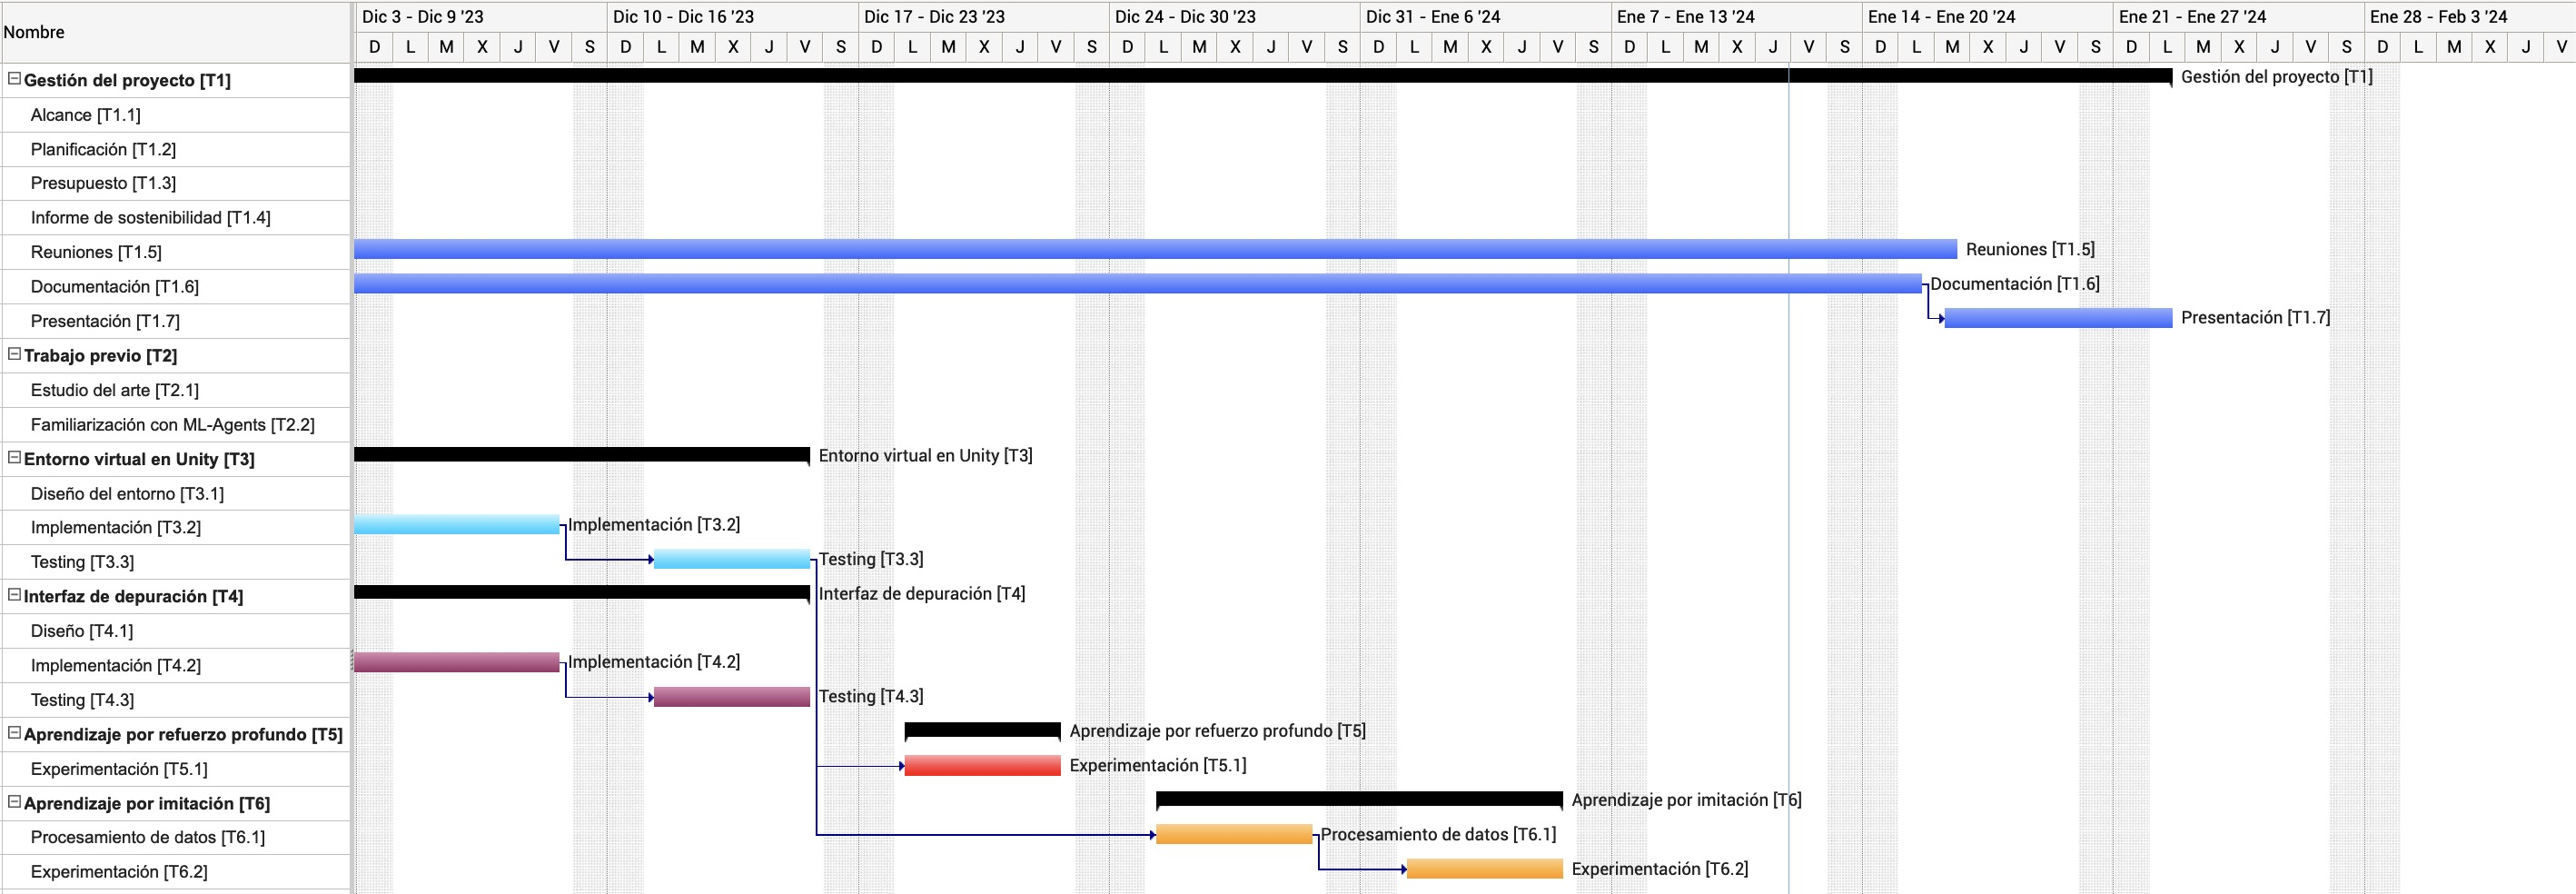
\includegraphics[width=\textwidth]{figures/gantter2-final.jpg}
\caption[Diagrama de Gantt de la planificación final, parte 2 de 2]{Diagrama de Gantt de la planificación final, parte 2 de 2. (Elaboración propia)}
\label{fig:gantter2-fial}
\end{figure}

\chapter{Configuraciones del entrenamiento}
\section{Configuración del entrenamiento mediante PPO} \label{appendix:config-file-ppo}

\begin{verbatim}
behaviors:
  PadelAgent:
    trainer_type: ppo
    summary_freq: 25000
    max_steps: 1000000
    keep_checkpoints: 5
    hyperparameters:
      learning_rate: 0.0003
      learning_rate_schedule: linear
      batch_size: 512
      buffer_size: 20480
      beta: 0.005
      beta_schedule: linear
      epsilon: 0.2
      epsilon_schedule: linear
      num_epoch: 3
    network_settings:
      hidden_units: 64
      num_layers: 4
    reward_signals:
      extrinsic:
        gamma: 0.95
        strength: 1.0
    self_play:
          save_steps: 50000
          swap_steps: 25000
          team_change: 200000
          window: 15
          play_against_latest_model_ratio: 0.5
          initial_elo: 1200.0
\end{verbatim}

\newpage
\section{Configuración del entrenamiento mediante PPO + Curiosity} \label{appendix:config-file-curiosity}
\begin{verbatim}
behaviors:
  PadelAgent:
    trainer_type: ppo
    summary_freq: 25000
    max_steps: 1000000
    keep_checkpoints: 5
    hyperparameters:
      learning_rate: 0.0003
      learning_rate_schedule: linear
      batch_size: 512
      buffer_size: 20480
      beta: 0.005
      beta_schedule: linear
      epsilon: 0.2
      epsilon_schedule: linear
      num_epoch: 3
    network_settings:
      hidden_units: 64
      num_layers: 4
    reward_signals:
      extrinsic:
        gamma: 0.95
        strength: 1.0
      curiosity:
        gamma: 0.95
        strength: 0.05
        learning_rate: 1e-4
        network_settings:
          hidden_units: 128
          num_laters: 2
    self_play:
          save_steps: 50000
          swap_steps: 25000
          team_change: 200000
          window: 15
          play_against_latest_model_ratio: 0.5
          initial_elo: 1200.0
\end{verbatim}
